\documentclass[12pt]{article}
\usepackage{../lp,graphicx,amsmath}
\usepackage{tkz-berge}
% Cross-references for handout numbers.
\usepackage{amsfonts}
%\usepackage{amsthm}
\usepackage{hyperref}
\usepackage{amssymb}
%\usepackage[capitalize]{cleveref}
\usepackage{xcolor}

%\input{handouts}

\newcounter{chapnum}

\newtheorem{definition}{Definition}[chapnum]
\newtheorem{remark}{Remark}[chapnum]
\newtheorem{theorem}{Theorem}[chapnum]
\newtheorem{lemma}[theorem]{Lemma}
\newtheorem{corollary}[theorem]{Corollary}
\newtheorem{proposition}[theorem]{Proposition}
\newtheorem{claim}[theorem]{Claim}
\newtheorem{observation}{Observation}[chapnum]

\renewcommand{\thesection}{\arabic{chapnum}.\arabic{section}}
\renewcommand{\thefigure}{\arabic{chapnum}.\arabic{figure}}


\newenvironment{proof}{\noindent{\bf Proof:} \hspace*{1em}}{
        \hspace*{\fill} $\triangle$ }
\newenvironment{proof_of}[1]{\noindent {\bf Proof of #1:}
        \hspace*{1em} }{\hspace*{\fill} $\triangle$ }
\newenvironment{proof_claim}{\begin{quotation} \noindent}{
        \hspace*{\fill} $\diamond$ \end{quotation}}
\newenvironment{solution}{\noindent{\bf Solution:} \hspace*{1em}}{
        \hspace*{\fill} $\triangle$ }


\newcommand{\R}{{\mathbb R}}
\newcommand{\Z}{{\mathbb Z}}
\newcommand{\Q}{{\mathbb Q}}
\newcommand{\C}{{\mathbb C}}
\newcommand{\N}{{\mathbb N}}
\newcommand{\lin}{\operatorname{lin}}
\newcommand{\aff}{\operatorname{aff}}
\newcommand{\cone}{\operatorname{cone}}
\newcommand{\conv}{\operatorname{conv}}
\newcommand{\vol}{\operatorname{vol}}
\newcommand{\poly}{\operatorname{poly}}




\newcommand{\CF}[1]{{\color{purple}[CF: #1]}}


\newlength{\toppush}
\setlength{\toppush}{2\headheight}
\addtolength{\toppush}{\headsep}

\newcommand{\htitle}[2]{\noindent\vspace*{-\toppush}\newline\parbox{6.5in}
{Massachusetts Institute of Technology \hfill 18.453: Combinatorial Optimization 
\newline
\textbf{Instructor:} Cole Franks \quad \textbf{Notes: }Michel Goemans and Zeb Brady \hfill#2\newline
\mbox{}\hrulefill\mbox{}}\vspace*{1ex}\mbox{}\newline
\begin{center}{\Large\bf #1}\end{center}}

\newcommand{\handout}[2]{\thispagestyle{empty}
 \markboth{ #1 \hfil #2}{ #1 \hfil #2}
 \pagestyle{myheadings}\htitle{#1}{#2}}


\setlength{\oddsidemargin}{0pt}
\setlength{\evensidemargin}{0pt}
\setlength{\textwidth}{6.5in}
\setlength{\topmargin}{0in}
\setlength{\textheight}{8.5in}


\newcounter{exercisenum}
\newcounter{exercisetot}
\setcounter{exercisetot}{0}



\newenvironment{exercises}{
	\begin{list}{{\bf Exercise \arabic{chapnum}-\arabic{exercisenum}. \hspace*{0.5em}}}
	{\setlength{\leftmargin}{0em}
	 \setlength{\rightmargin}{0em}
	 \setlength{\labelwidth}{0em}
	 \setlength{\labelsep}{0em}
	\usecounter{exercisenum}
      \setcounter{exercisenum}{\theexercisetot}}}{\setcounter{exercisetot}{\theexercisenum}\end{list}}


\newenvironment{pseudocode}{
    \begin{list}{}{
        \renewcommand{\makelabel}{$\triangleright$}
        \setlength{\topsep}{0pt}
        \setlength{\leftmargin}{32pt}
        \setlength{\labelwidth}{14pt}
        \setlength{\labelsep}{0mm}
        \setlength{\itemindent}{0mm}
        \setlength{\itemsep}{-3pt}
        \setlength{\itemsep}{0mm}
        \setlength{\parsep}{0pt}%
        \setlength{\listparindent}{0pt}
    }
}
{
    \end{list}
}

\setlength{\topmargin}{-1in}
\setlength{\textheight}{9.7in}
%\usepackage{epsfig}

\begin{document}

%\handout{QUIZ 1}{April 11th, 2017}

\noindent {\Large 18.453 Quiz} \\
~\\

\paragraph{Instructions.} This is both an {\bf in-class} quiz  and a {\bf take-home} quiz. For the {\it in-class} quiz, answer the following questions in the blue booklet and hand in the booklet at the end of the quiz (3:55PM on April 9th, 2019). Then take the questions home, and you should answer them again by the beginning of class on Thursday April 18th. For the  take-home part, you can consult the lecture notes and other material, but you are not allowed to discuss it with your friends. Please write the solutions to the {\bf take-home} as {\bf neatly} as possible, and show your steps. Your grade will be the average of these two grades. 


\begin{enumerate}
\item
\begin{enumerate}
\item
Given a bipartite graph,  state K\"onig's theorem about the size of the maximum matching in $G$. 
\item  
Find a minimum vertex cover in the following
graph, and give a short argument for its optimality. 

%\begin{center}
%\includegraphics{mat1}
%\end{center}

%vertex cover: a0, a1, b1, a3
%matching: a0b0, a1b2, a3b3, a4b1
\begin{center}
\begin{tikzpicture}
   \begin{scope}[rotate=90]
       \SetVertexMath
       \grEmptyLadder[RA=-2,RB=-4]{5}   
   \end{scope}
    \Edges(a0,b0,a1,b2,a3,b3,a1)
    \Edges(a4,b1)
    \Edges(b1,a2)
    \Edges(a1,b4,a3)
    \Edges(b1,a0,b2)
\end{tikzpicture}
\end{center}
\end{enumerate}
%%%%%%%%%%%%%%%%%

\newpage
\item
An $n\times n$ matrix $A$ is called \emph{doubly stochastic} if all the entries of $A$ are nonnegative, and if the entries of every row and column of $A$ sum to $1$.
\begin{enumerate}
\item Define a bipartite graph $G_A$ on with vertex sets $\{a_1, ..., a_n\}$ and $\{b_1, ..., b_n\}$, and with an edge connecting $a_i$ to $b_j$ whenever $A_{ij} > 0$. Show that if $A$ is doubly stochastic, then $G_A$ has a perfect matching.

\item Show that every $n\times n$ doubly stochastic matrix can be written as a convex combination of at most $n^2$ permutation matrices.

\item ({\bf Extra Credit}) Can the number $n^2$ in part (b) be reduced? If so, how much can you reduce it?
\end{enumerate}

\newpage
\item
%Suppose that we have a (general, i.e. not necessarily bipartite) graph $G=(V,E)$, and we have two matchings $M_1$ and $M_2$ in $G$. Let $V_1=V(M_1)$ and $V_2=V(M_2)$ be the  vertices matched by these two matchings. Thus, $|V_1|=2|M_1|$ and $|V_2|=2|M_2|$.  Show that if $|V_1|>|V_2|$ then there exists a matching $M_3$ covering $V_2$ and also at least one 
%vertex of $V_1\setminus V_2$. 
Suppose $G = (V,E)$ is a $2$-edge-connected graph (that is, $G$ remains connected if you delete any single edge) with at least one perfect matching, and suppose that $G$ has a special edge $e$ which shows up in \emph{every} perfect matching of $G$. Show that there is necessarily a nonempty set $S \subseteq V$ with the following properties:
\begin{itemize}
\item the number of odd components of $G\setminus S$ is exactly $|S|$,

\item $G\setminus S$ has at least one even component.
\end{itemize}


%\newpage
%\item
%Consider a directed graph $G=(V,E)$ with vertices $s, t\in V$. Assume there exists an integer flow $x: E\rightarrow \Z$ from $s$ to $t$ of value $2k$ with $0 \leq x_e \leq k$ for all $e\in E$. 
%\begin{enumerate}
%\item
%Show that there exists $F\subseteq E$ such that (i) every edge $e$ with $x_e=k$ is in $F$ (i.e. $\{e: x_e=k\}\subseteq F$), (ii) no edge with $x_e=0$ is in $F$, and (iii) the vector $y$ with $y_e=1$ for $e\in F$ and $y_e=0$ for $e\notin F$ is a flow of net value 2 from $s$ to $t$. 
%\item
%Assuming part (a), show that the flow $x$ can be decomposed into the sum of $k$ {\it integer} flows $y^{(1)}, \cdots, y^{(k)}$ each of value $2$ from $s$ to $t$. This means that for all $e$ we have 
%$$x_e=\sum_{i=1}^k y^{(i)}_e. $$
%\end{enumerate}

%%%%%%%%%%%%%%%%%%%%%%
\newpage
\item
Given a {\it bipartite} graph $G=(V,E)$ with bipartition $V=A \cup B$
and given an integer $k$, consider the set of all matchings of
cardinality at most $k$. We know that if there was no constraint on
the cardinality (for example, if $k\geq |V|/2$) then the convex hull $P$
of all (incidence vectors of) matchings would be given by
$$ \begin{array}{ll@{\hspace{0.5in}}l}
P=\{ x\in \R^{|E|}: & \displaystyle \sum_{j\in B: (i,j)\in E} x_{ij}
\leq 1 & i \in A \\
& \displaystyle \sum_{i\in A: (i,j)\in E} x_{ij}
\leq 1 & j \in B \\
 & x_{ij}\geq 0 & (i,j)\in E \} \end{array}$$

In this exercise, you will show that the convex hull $P_k$ of all
matchings of cardinality at most $k$ is  given by 
$$ \begin{array}{lll}
P_k=\{ x\in \R^{|E|}: & \displaystyle \sum_{j\in B: (i,j)\in E} x_{ij}
\leq 1 & i \in A \\
& \displaystyle \sum_{i\in A: (i,j)\in E} x_{ij}
\leq 1 & j \in B \\
& \displaystyle \sum_{(i,j)\in E} x_{ij} \leq k \\
 & x_{ij}\geq 0 & (i,j)\in E \} \end{array}$$
Here are three ways to prove it. Do {\bf just one} of them for the in-class quiz for full credit (I would suggest doing the first one), but do {\bf two} of them for the take-home version. 

\begin{enumerate}
\item
Show that the underlying matrix $A$ is totally unimodular, where $P_k
=\{x: Ax\leq b, x\geq 0\}$. If you use this way, first define what a
totally unimodular matrix is, specify what the matrix $A$ look like, and explain why this implies the description of $P_k$. 
\item
Provide a reduction between matchings of cardinality at most $k$ in $G$ and feasible integer flows (of any value) between two vertices $s$ and $t$ in an augmented graph $G'$. Explain why this would imply the integrality of the description of $P_k$. 
\item
Consider any vertex $x^*$ of $P_k$. First argue that $x^*$ is in a face of
dimension 1 of $P$ (the matching polytope without restriction on the
cardinality), i.e. $x^*$ can be seen as a convex combination of
incidence vectors of 
two {\it adjacent} matchings $M_1$ and $M_2$ of $G$. Then state
(without proof) the
condition for two matchings $M_1$ and $M_2$ to be adjacent on
$P$. Finally conclude that $x^*$ must have been the incidence vector
of either $M_1$ or  $M_2$. 
\end{enumerate}


\newpage
\item
({\bf Take-home only problem}) Consider a directed graph $G = (V,E)$ with vertices $s,t \in V$ and capacities $u(e)$ for each edge $e \in E$. Define the \emph{flow polytope} to be the set
\[
\begin{array}{lrl}
P=\{ x\in \R^{|E|}: & \displaystyle \sum_{e\in \delta^+(u)} x_e - \sum_{e\in \delta^-(u)} x_e = 0 & u\in V\setminus\{s,t\} \\
& 0 \leq x_e \leq u(e) & e\in E \}. \end{array}
\]
Suppose we start with a (non-maximal) flow $x$ which corresponds to a \emph{vertex} of this flow polytope $P$, find an augmenting path from $s$ to $t$, compute the bottleneck for this path, and push that much flow along the augmenting path to make an augmented flow $x'$. Does the augmented flow $x'$ necessarily correspond to a vertex of the flow polytope $P$?









\end{enumerate}
\end{document}
